\section{Additional flow fields and vortex diagnostics}
\label{suppsec:fields}

\subsection{Additional fields}

Figures~\ref{suppfig:fields_alpha0} and~\ref{suppfig:fields_alpha01} collect all twenty-four converged configurations at $N=384$, split by amplitude: $\alpha=0$ and $\alpha=0.1$, respectively. Presenting the two amplitudes in separate figures ensures that undulated and non-undulated cases are never superposed for the same geometry. In each figure the rows correspond to $Re=100$, $400$, and $1000$ and the columns to the full exponent sequence $n=2,4,6,8$, so that every panel is filled. The main manuscript (Fig.~3) shows the $Re=400$ row of both amplitudes at a larger panel size; the present figures extend that selection to the two remaining Reynolds numbers without mixing amplitudes. Within each figure all panels share one colour scale, set by the largest velocity magnitude over its twelve configurations.

\begin{figure}[!htbp]
\centering
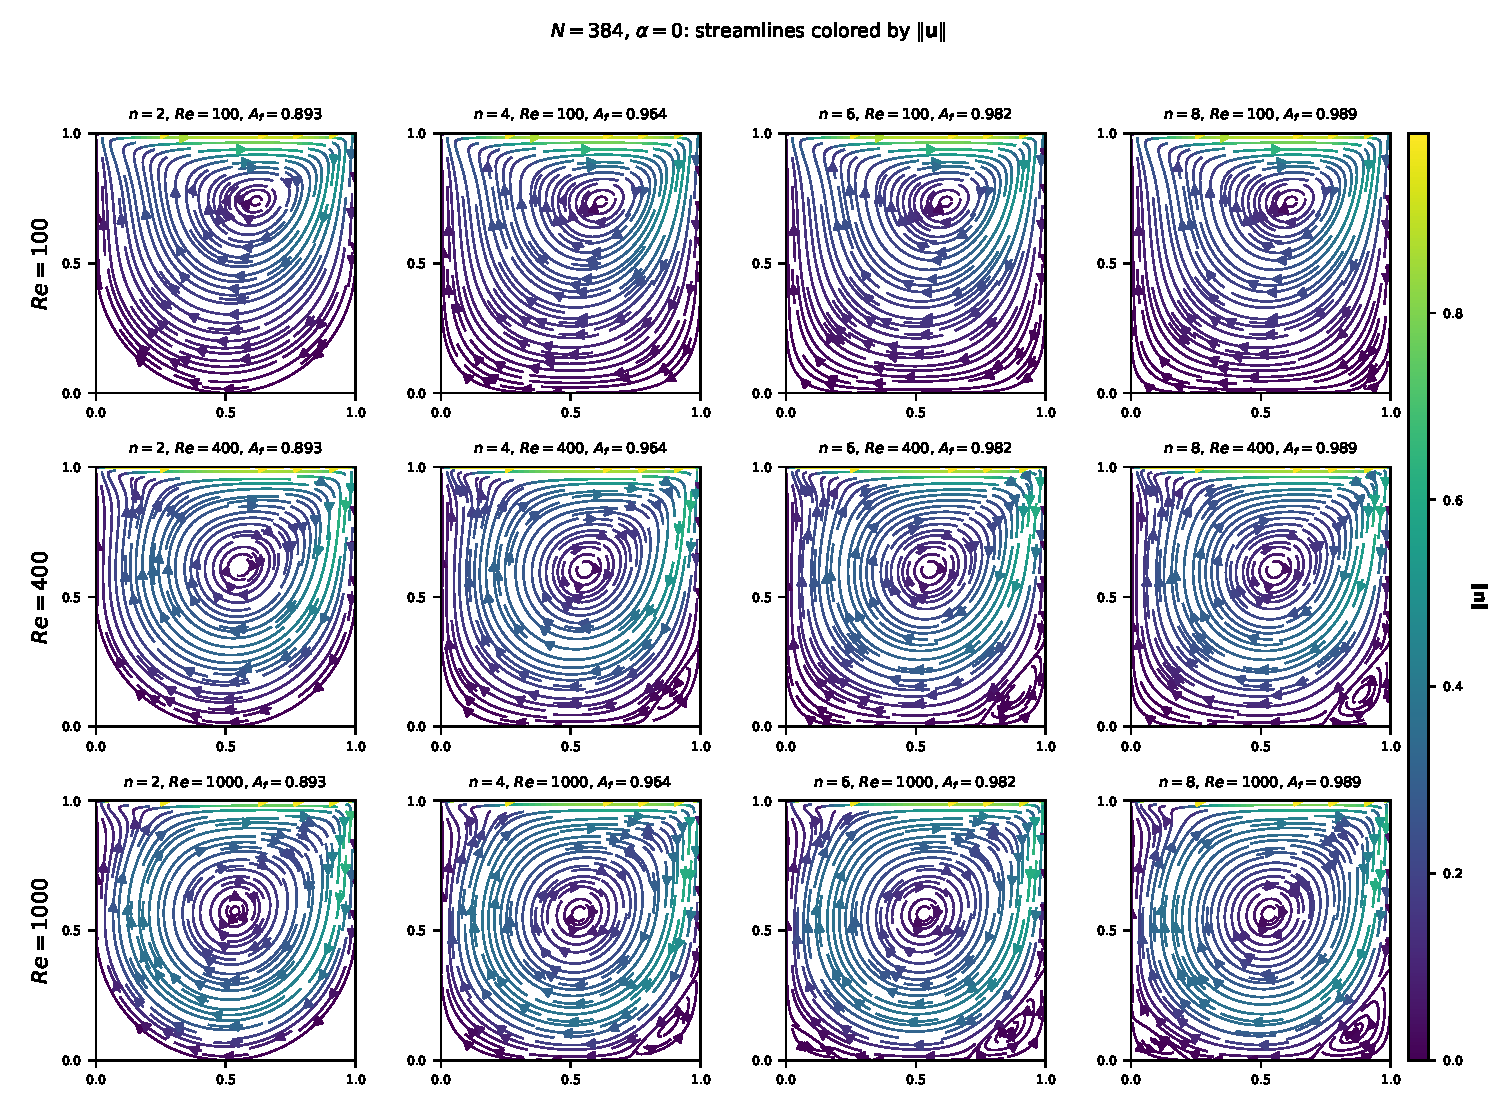
\includegraphics[width=0.95\columnwidth]{figures/figS_fields_alpha0.pdf}
\caption{Streamlines colored by velocity magnitude for the twelve converged $\alpha=0$ configurations at $N=384$. Rows: $Re=100$, $400$, $1000$; columns: $n=2$, $4$, $6$, $8$. Each panel is labeled with its exponent, Reynolds number and fluid area $A_f$, and the color scale is common to all panels of the figure.}
\label{suppfig:fields_alpha0}
\end{figure}

\begin{figure}[!htbp]
\centering
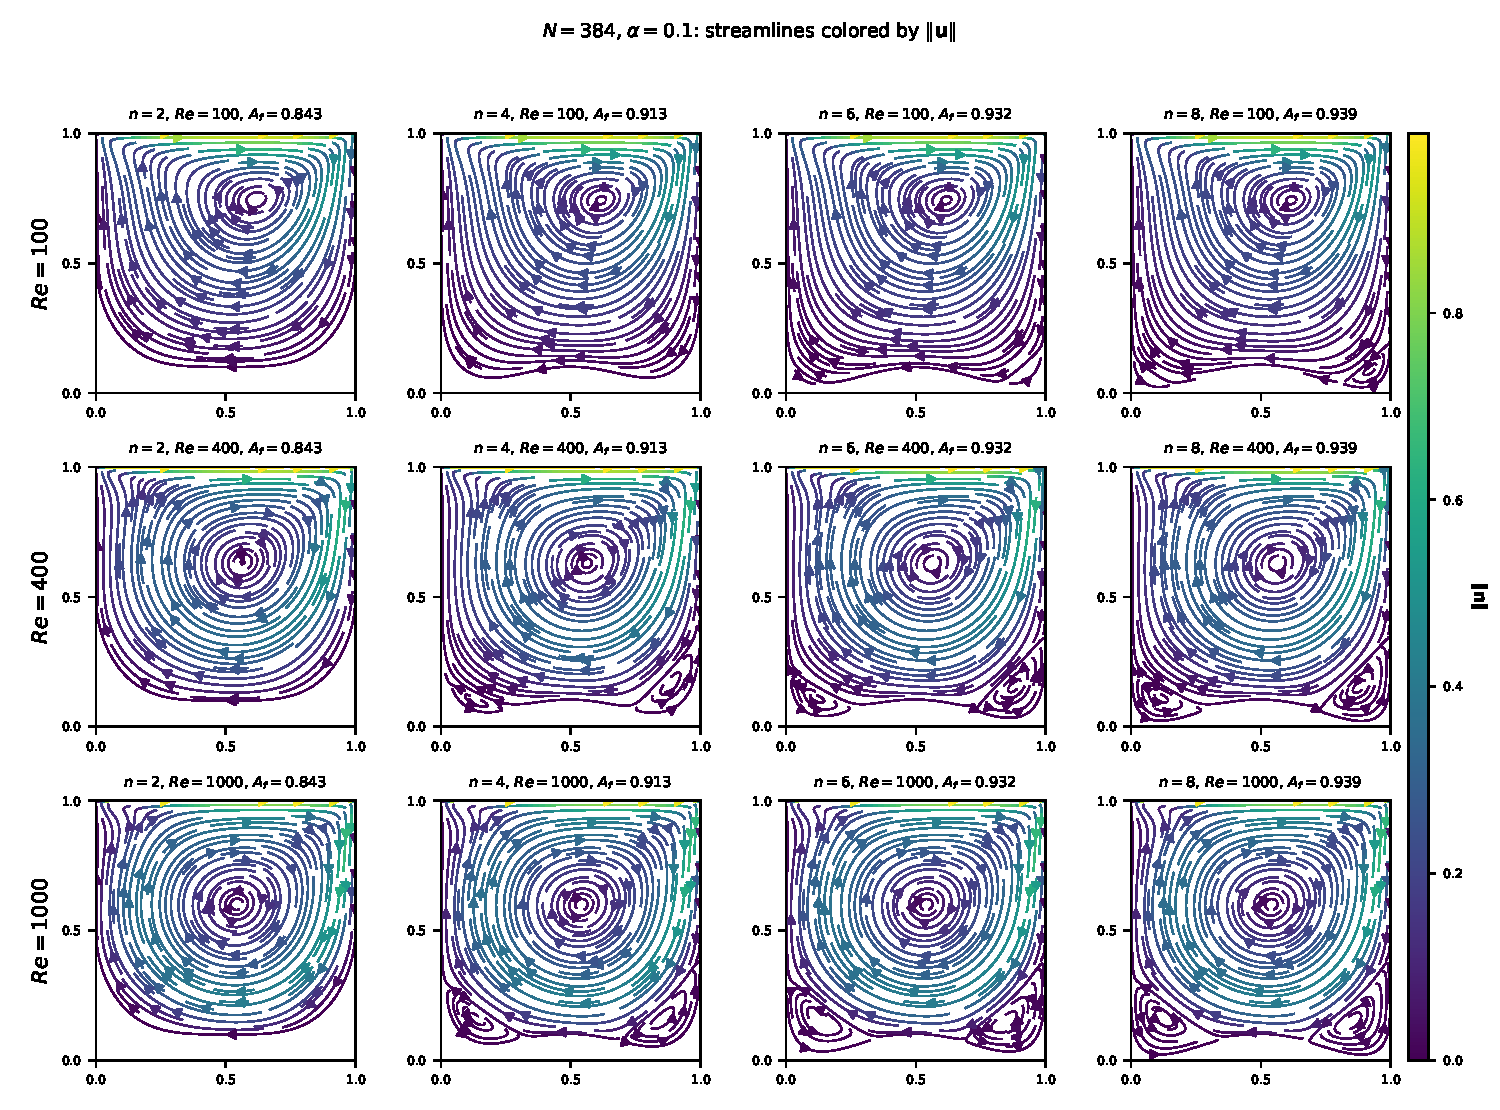
\includegraphics[width=0.95\columnwidth]{figures/figS_fields_alpha01.pdf}
\caption{Same as Fig.~\ref{suppfig:fields_alpha0} for $\alpha=0.1$. The undulated cases are kept separate from the non-undulated fields of Fig.~\ref{suppfig:fields_alpha0}; the wavy bottom wall and the corner vortices it nucleates at $Re\ge400$ are visible in every column.}
\label{suppfig:fields_alpha01}
\end{figure}

\subsection{Vortex diagnostics}

Vortex locations and counts were extracted from the converged fields using a simple critical-point detection: the velocity gradient tensor is evaluated at each grid point, and points where both velocity components vanish (within a tolerance) are classified as centers or saddles. The primary vortex is identified as the center with the largest circulation. This diagnostic is used qualitatively in the main text; a complete vortex census is not included because the energetic contrasts are the primary focus of the analysis.
